\section{Results}

%For results talk about what you would measure.

To determine the results of the experiment, I would conduct the experiment on each cockroach. Ideally, I would have at least 10 healthy adult cockroaches to test on. For each experiment, I would use a timer to measure the time it took for a cockroach to react to the stimulation and the electrical tape to measure the angle of turn. 

% What else should I measure?

With the cockroaches that successfully turn left and right when stimulated, I will place them on track made of thin strips of electrical tape consisting of straight paths and \ang{90} turns and observe their ability to make it all the way through. I will also test the roach's ability to turn to various angles by modulating the current sent to its antennae and evaluating its performance of different maneuvers such as the Dieudonne Spiral, a siunsoid, and a zig-zag.

Assuming that I could control forward motion and the sharpness of the turn by modulating the current sent to the roach's antenna, I could evaluate performance through various maneuvers. For a counterclockwise Dieudonne Spiral, I would start by having the roach move forward in one direction. Then I would gently stimuate its right antenna, turning the roach to the left in slight increments of about 5 degrees every 2 seconds to achieve the large outer portion of the spiral. Once it has almost made a complete circle, I would stimulate its right antenna at a higher level, turning the roach in increments of about 15 degrees to achieve a smaller spiral. Then I would stimulate its right antenna at an even higher level, turning the roach in increments of about 30 degrees to achieve the smallest inner spiral.

For the sinusoid, I would execute a similar pattern of stimulation as the Dieudonne Sprial, but I would need to stimulate both antennae. I would start by having the roach move forward in one direction. Then I would stimuate its left antenna, turning the roach to the right by about 10 degrees. I would let the roach continue on the path until its position was nearly at my desired peak. Once the roach started to approach the peak of the sinusoid, I would stimulate its left antenna multiple times to achieve multiple right turns of about 30 degrees until it was on a downward path. I would let the roach continue on the downward path until its position was nearly at my valley. Once the roach started to approach the valley of the sinusoid, I would stimulate its right antenna multiple times to achieve multiple left turns of about 30 degrees until it was on an upward path again.

For the zig-zag, I would start by having the roach move forward in one direction. Then I would sharply stimuate its right antenna, turning the roach to the left by about 90 degrees. After letting the roach move forward in its new direction for about 5 seconds, I would sharply stimulate its left antenna, turning the roach to the right by about 90 degrees, letting it walk in its new direction for about 5 seconds before having it turn again.

Once directional control is achieved, I will try to achieve speed control. Stimulation to the antennae may not necessarily control speed in addition to direction, so I will attempt to stimulate other areas of the roach's body to change its speed. Figure \ref{fig:rough} displays the open and closed loop diagrams for the experiment, as well as sketches of maneuvers that can be performed to evaluate directional control.

{\begin{figure}[ht!]
\centering
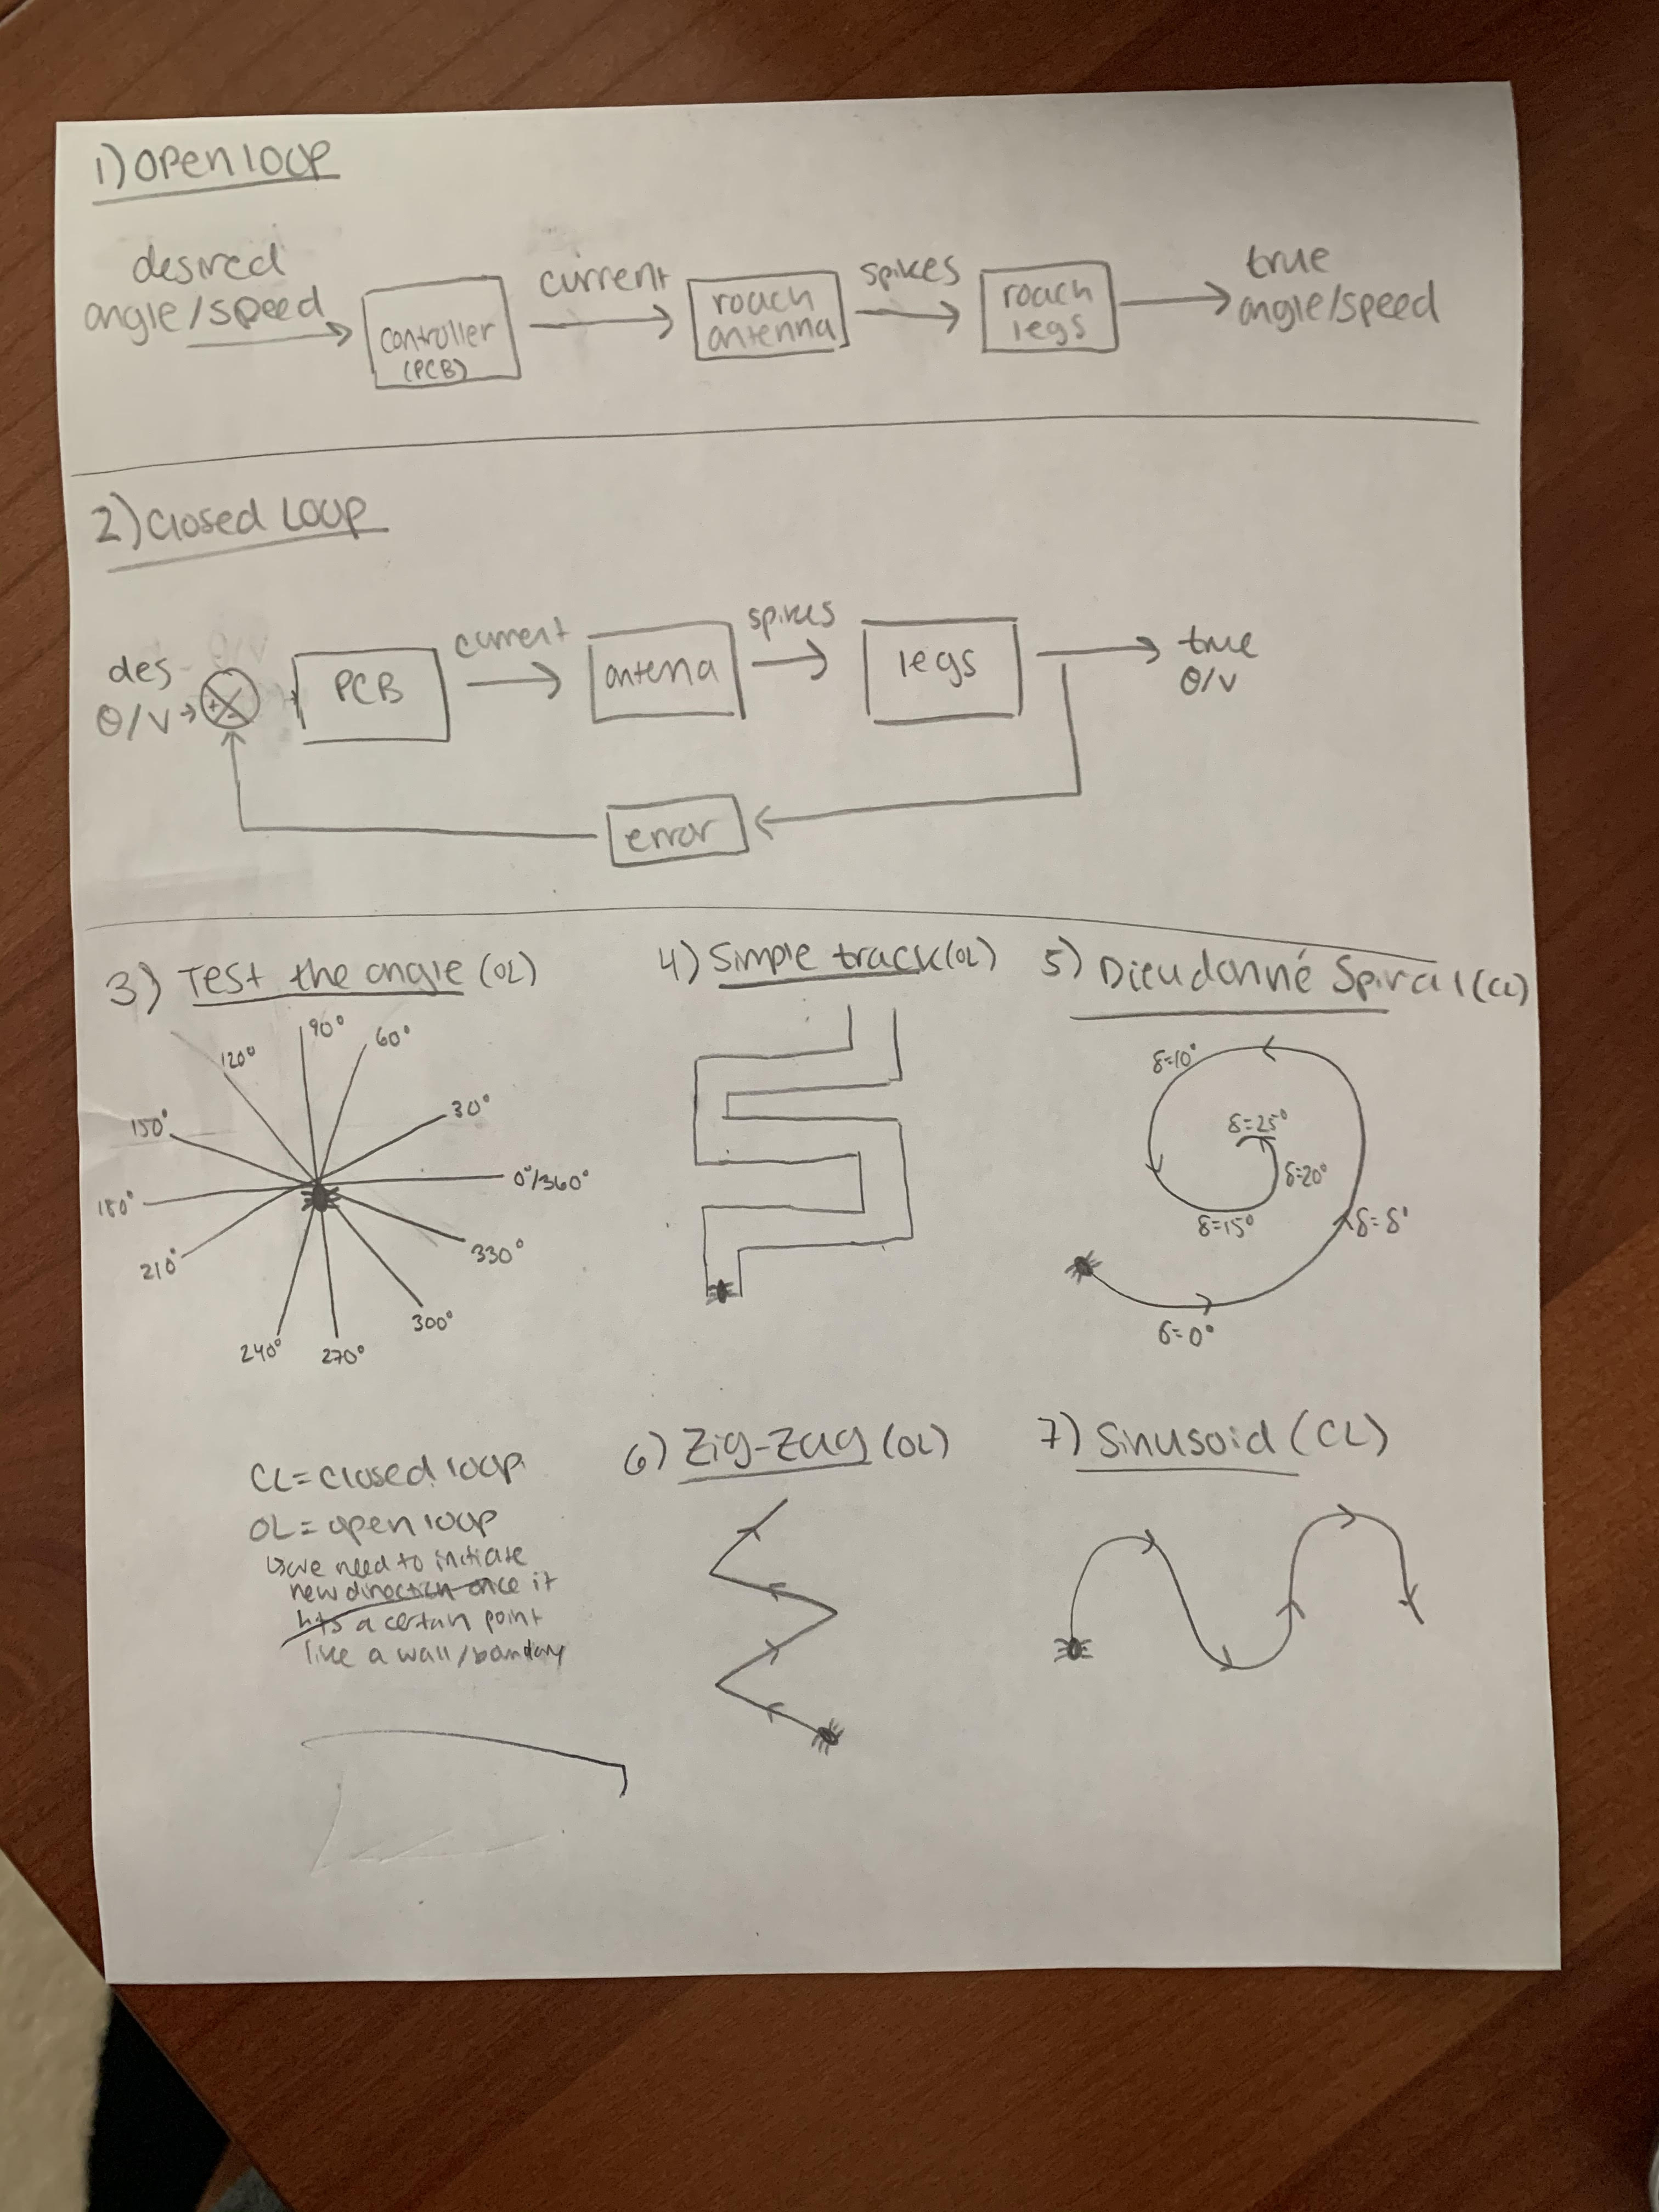
\includegraphics[scale=0.1]{Figures/OpenClosedLoops.jpg}
\caption{Open and Closed Loop Diagrams and Maneuvers}
\label{fig:rough}
\end{figure}}


 